\documentclass[xcolor=dvipsnames]{beamer}
\usepackage{subfig}
\usepackage{multimedia}
%\usecolortheme{blue}
%\definecolor{NVidiaGreen}{rgb}{0.4627, 0.7255, 0} % UBC Blue (primary)
\usecolortheme[named=gray]{structure}
\setbeamertemplate{caption}[numbered]
\usepackage[superscript,biblabel]{cite}
\title{Progressive Growing of GANs}
\author{Joris ten Tusscher}
\begin{document}



\frame{\titlepage}



\begin{frame}
\frametitle{The paper}
\begin{itemize}
	\item ``PROGRESSIVE GROWING OF GANS FOR IMPROVED QUALITY, STABILITY, AND VARIATION''\cite{karras2017progressive}
	\item Tero Karras, Timo Aila, Samuli Laine, Jaakko Lehtinen
	\item NVIDIA research
	\item Presented in 2018 at ICLR (International Conference on Learning Representations)
\end{itemize}
\end{frame}



\begin{frame}
\frametitle{Goal}
\begin{itemize}
	\item Generate new, realistic samples from a high-dimensional data distribution.
	\item \textbf{Example}: modelling the distribution of real images, and use that to generate new, real looking images.
\end{itemize}
\end{frame}



\begin{frame}
\frametitle{Approaches}
\begin{enumerate}
	\item Autoregressive (AR) models
	\item Variational Autoencoders (VAE)
	\item Generative Adversarial Network (GAN)
\end{enumerate}
\end{frame}



\begin{frame}
\frametitle{Approaches}
\begin{enumerate}
	\item \textbf{Autoregressive (AR) models}
	\item Variational Autoencoders (VAE)
	\item Generative Adversarial Network (GAN)
\end{enumerate}
\end{frame}



\begin{frame}
\frametitle{Autoregressive (AR) models}
\begin{itemize}
	\item Regression function: $X \rightarrow W \rightarrow \hat{y}$ 
		\begin{itemize}
			\item $X$: model input (list of independent variables $x_1$, $x_2$, ..., $x_n$).
			\item $W$: model coefficients $w_0$, $w_1, ..., w_n$.
			\item $\hat{y}$: prediction
			\item e.g. $\hat{y} = w_0 + w_1x_1 + w_2x_2^2 + w_3x_3^3 + ...$
		\end{itemize}
		\item Example: predict colloquium turn-out $\hat{y}$ based on time of day ($x_0$), day of week ($x_1$), number of subsequent colloquium talks ($x_2$).
	\item Autoregression:
		\begin{itemize}
			\item $X$ consists of observations from $n$ previous time steps.
			\item $\hat{y}$ is usually renamed to $\hat{x}_{n+1}$.
		\end{itemize}
\end{itemize}
\end{frame}



\begin{frame}
\frametitle{PixelCNN (AR image generator model)\cite{pixelcnn} (2016)}
\begin{itemize}
	\item model joint distribution of pixels over an image $X$ as product of conditional distributions:
	
	$p(X) = \prod_{i=1}^{n^2} p\left(x_i | x_1, \ldots , x_{i-1} \right)$
	\item Gives sharp images, but obviously \textbf{very} slow (one neural network per pixel!).
\end{itemize}
\end{frame}



\begin{frame}
\frametitle{PixelCNN (AR image generator model)\cite{pixelcnn} (2016)}
\begin{itemize}
	\item model joint distribution of pixels over an image $X$ as product of conditional distributions:
	
	$p(X) = \prod_{i=1}^{n^2} p\left(x_i | x_1, \ldots , x_{i-1}\right)$
	\item Gives sharp images, but obviously \textbf{very} slow (one neural network per pixel!).
	\item Add extra dependencies, e.g. \textbf{latent representation} F of some random input image:

	$p(X) = \prod_{i=1}^{n^2} p\left(x_i | x_1, \ldots , x_{i-1}, \mathbf{F} \right)$
\end{itemize}
\end{frame}



\begin{frame}
\frametitle{Latent representations}
\begin{itemize}
	\item Latent space is intermediate representation in autoencoder.
	\item Autoencoder:
	\begin{itemize}
		\item $\phi : X \rightarrow F$
		\item $\psi : F \rightarrow X$
		\item $\phi , \psi = \underset { \phi , \psi } { \arg \min } \| X - ( \psi \circ \phi ) X \| ^ { 2 }$
		\item Visualised:
			\begin{figure}
			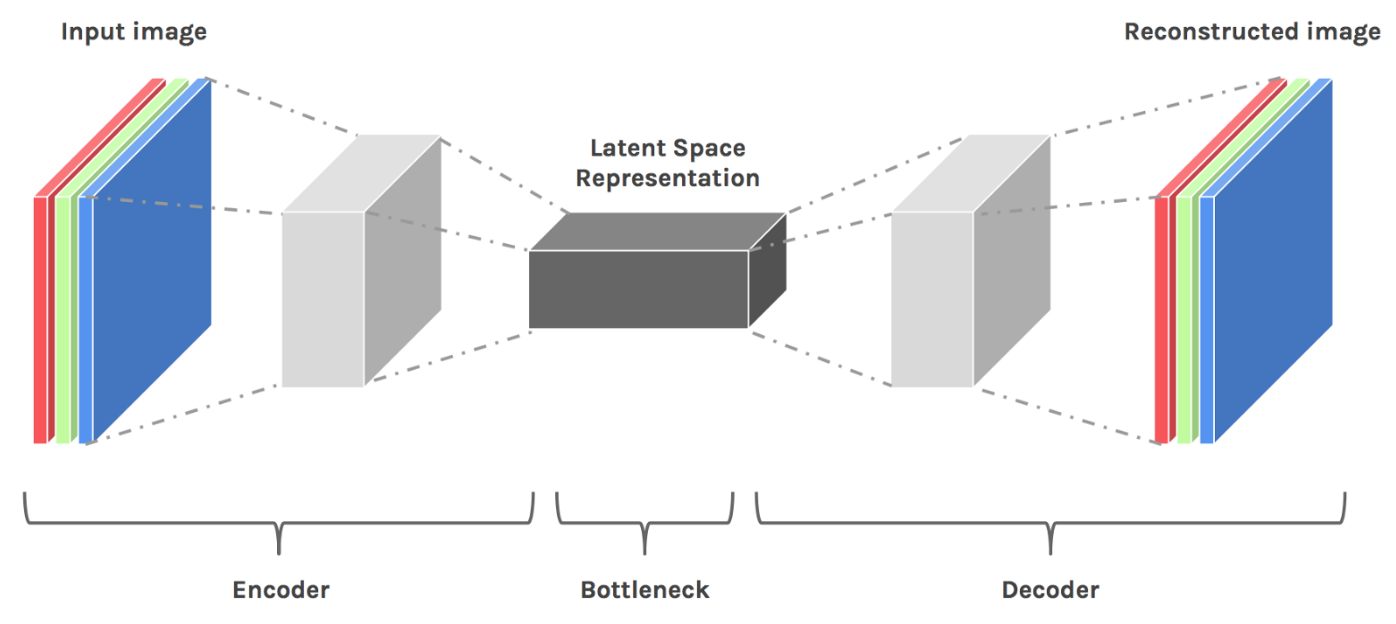
\includegraphics[width=\linewidth]{img/autoenc.png}	
			\end{figure}
	\end{itemize}
\end{itemize}
\end{frame}



\begin{frame}
\frametitle{PixelCNN (AR image generator model)\cite{pixelcnn} (2016)}
\begin{figure}
	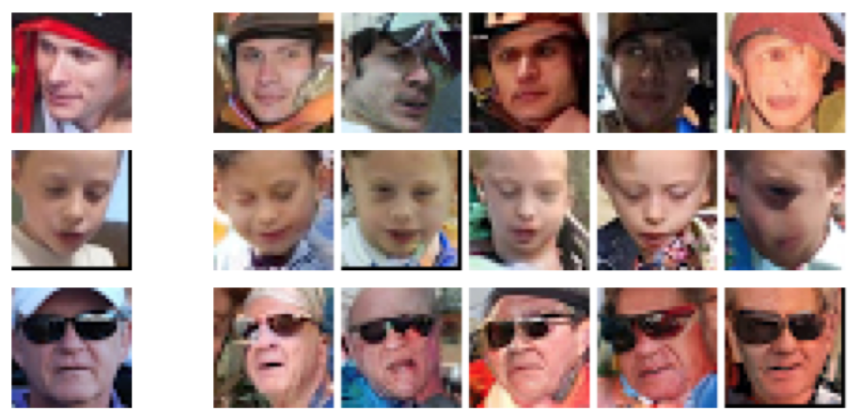
\includegraphics[width=\linewidth]{img/pixelcnn_small.png}
	\caption{Images generated using PixelCNN\cite{pixelcnn} with extra constraint from latent space.}
\end{figure}
\end{frame}



\begin{frame}
\frametitle{Approaches}
\begin{enumerate}
	\item \textbf{Autoregressive (AR) models}
	\item Variational Autoencoders (VAE)
	\item Generative Adversarial Network (GAN)
\end{enumerate}
\end{frame}



\begin{frame}
\frametitle{Approaches}
\begin{enumerate}
	\item Autoregressive (AR) models:
		\begin{itemize}
			\item High quality
			\item Extremely slow
		\end{itemize}
	\item \textbf{Variational Autoencoders (VAE)}
	\item Generative Adversarial Network (GAN)
\end{enumerate}
\end{frame}



\begin{frame}
\frametitle{Variational Autoencoders (VAE)}
\begin{itemize}
	\item Recall the AE:
		\begin{figure}
		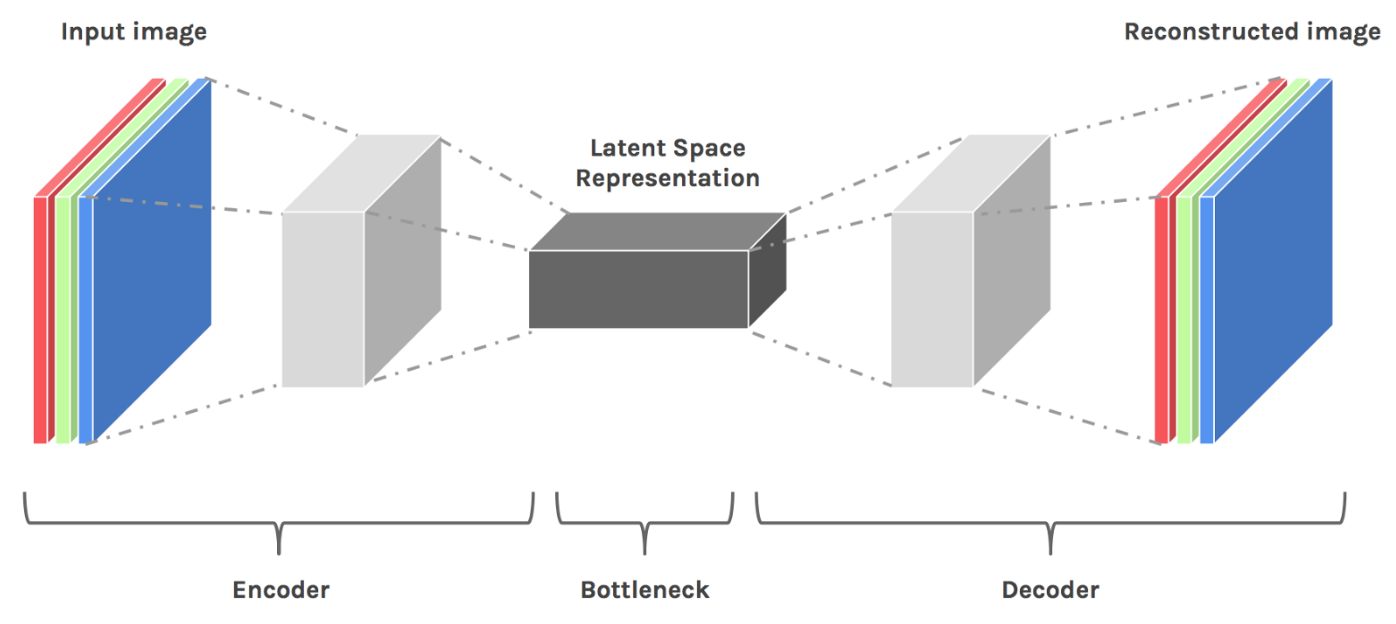
\includegraphics[width=\linewidth]{img/autoenc.png}	
		\end{figure}
	\item Observation: we know nothing about the latent space distribution.
	\item Fix: force encoder to generate vectors that roughly follow certain distribution (e.g. isotropic multivariate $\mathcal{N}(\mu=0$, $\sigma^2=1)$).
\end{itemize}
\end{frame}



\begin{frame}
\frametitle{Variational Autoencoders (VAE)}
\begin{itemize}
	\item Fast generation: only 1 neural network
	\item Blurry output due to latent space distribution constraint
\end{itemize}
\begin{figure}
	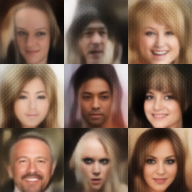
\includegraphics[width=0.5\linewidth]{img/vae_small.png}
\end{figure}
\end{frame}



\begin{frame}
\frametitle{Approaches}
\begin{enumerate}
	\item Autoregressive (AR) models:
		\begin{itemize}
			\item High quality
			\item Extremely slow
		\end{itemize}
	\item \textbf{Variational Autoencoders (VAE)}
	\item Generative Adversarial Network (GAN)
\end{enumerate}
\end{frame}



\begin{frame}
\frametitle{Approaches}
\begin{enumerate}
	\item Autoregressive (AR) models:
		\begin{itemize}
			\item High quality
			\item Extremely slow
		\end{itemize}
	\item Variational Autoencoders (VAE)
		\begin{itemize}
			\item Blurry
			\item Fast
		\end{itemize}
	\item \textbf{Generative Adversarial Network (GAN)}
\end{enumerate}
\end{frame}



\begin{frame}
\frametitle{Generative Adversarial Networks}
\begin{itemize}
	\item Proposed in 2014 by Goodfellow et al.\cite{goodfellow2014generative}
	\item A GAN is a two player minimax game:
		\begin{itemize}
			\item Generator \textbf{G} captures data distribution
			\item Discriminator \textbf{D} discriminates between training data and data from G.
		\end{itemize}
	\item G and D constantly try to beat each other.
\end{itemize}
\end{frame}



\begin{frame}
\frametitle{On $G$ and $D$}
\begin{itemize}
	\item \textbf{$G$}enerator can be any arbitrary function $Z \rightarrow X$
		\begin{itemize}
			\item $Z$: noise vector
			\item $X$: output (in our context: image)
		\end{itemize}
	\item \textbf{$D$}iscriminator can be any arbitrary function $X \rightarrow P$
		\begin{itemize}
			\item $P$: probability that $X$ comes from real data and not $G$.
		\end{itemize}
\end{itemize}
\end{frame}



\begin{frame}
\frametitle{The minimax game}
\begin{itemize}
	\item For $D$: maximise probability that $D$ predicts correct class for random inputs.
	\item For $G$: minimise $1 - D(G(Z))$.
	\item Formally: let's say that $V(D,G)$ is the valuation function of our minimax game, then:\\\

$\underset{G}{min}\ \underset{D}{max}\ V(D, G) = \mathbb{E}_{X \sim p_{data}(X)}[\log D(X)]$
	
	\begin{enumerate}[]
		\item $\ \ \ \ \ \ \ \ \ \ \ \ \ \ \ \ \ \ \ \ +\ \mathbb{E}_{Z \sim p_Z(Z)}[\log(1 - D(G(Z)))]$
	\end{enumerate}
\end{itemize}
\end{frame}



\begin{frame}
\frametitle{How to train GANs?}
\begin{itemize}
	\item How to train NNs in general?
	\begin{itemize}
		\item Realise that loss of NN is function $\mathcal{L}$ of network parameters $\theta$
		\item Calculate gradient $\nabla \mathcal{L}$
		\item Move in opposite direction of $\nabla \mathcal{L}$
		\item But don't actually do this.
	\end{itemize}
\end{itemize}
\begin{center}
	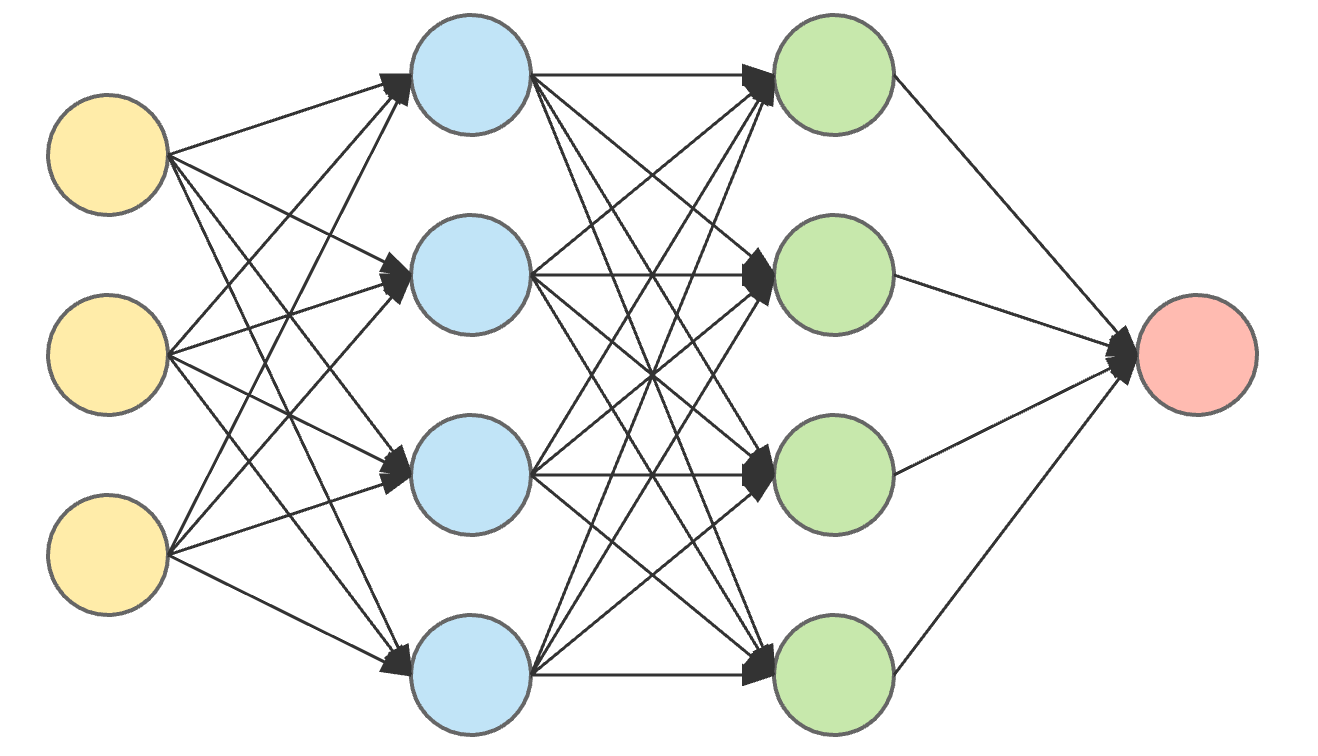
\includegraphics[width=0.5\textwidth]{img/NN_small.png}%
	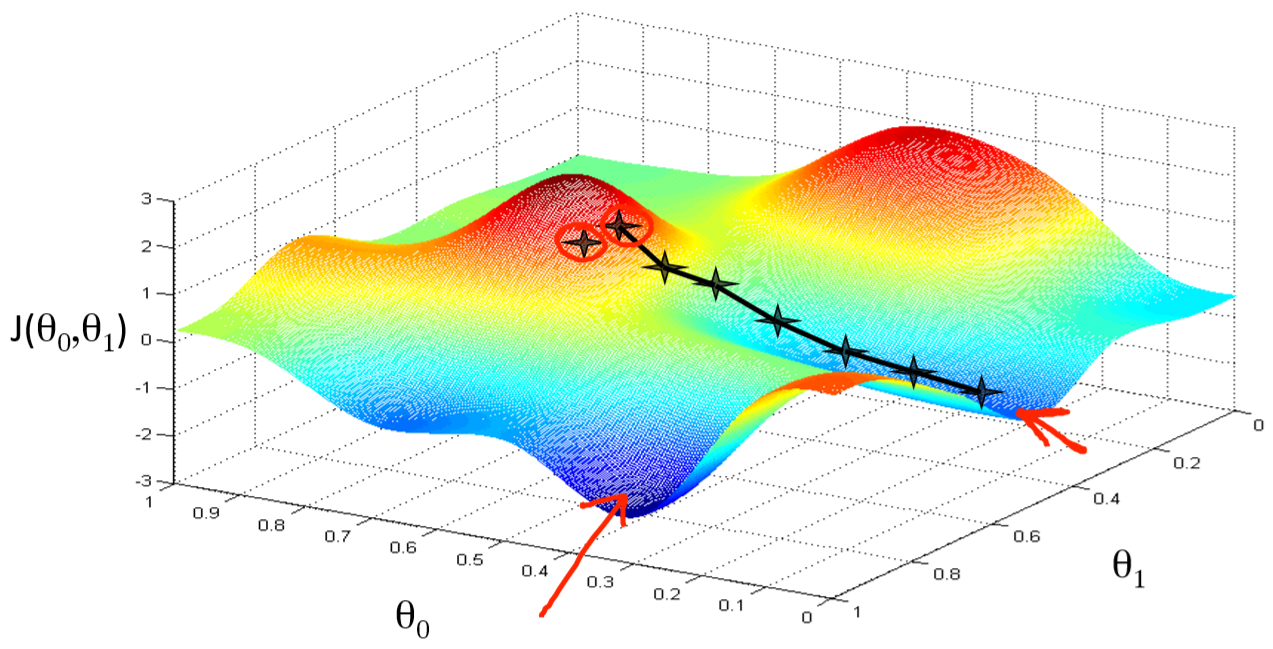
\includegraphics[width=0.5\textwidth]{img/grad_desc.png}
\end{center}
\end{frame}



\begin{frame}
\frametitle{Iteratively training a GAN\cite{goodfellow2014generative}: training algorithm}

\begin{enumerate}
	\item Repeat until happy
	\begin{enumerate}
		\item Build minibatch $Z$ of $m$ noise samples $\{z^{(1)}, \ldots, z^{(m)}\}$ using $p_Z$
		\item Build minibatch $X$ of $m$ data samples $\{x^{(1)}, \ldots, x^{(m)}\}$ using $p_{data}$
		\item Update $D$ by \underline{a}scending its stochastic gradient:
		$\nabla _ { \theta _ { d } } \frac { 1 } { m } \sum _ { i = 1 } ^ { m } \left[ \log D( x ^ { ( i ) } ) + \log \left( 1 - D \left( G \left( z ^ { ( i ) } \right) \right) \right) \right]$
		\item Resample $Z$.
		\item Update $G$ by \underline{de}scending its stochastic gradient:
		$\nabla _ { \theta _ { g } } \frac { 1 } { m } \sum _ { i = 1 } ^ { m } \log \left( 1 - D \left( G \left( \boldsymbol { z } ^ { ( i ) } \right) \right) \right)$	
	\end{enumerate}
\end{enumerate}

\end{frame}



\begin{frame}
\frametitle{Iteratively training a GAN\cite{goodfellow2014generative}: training algorithm visualisation}
\begin{figure}
\center
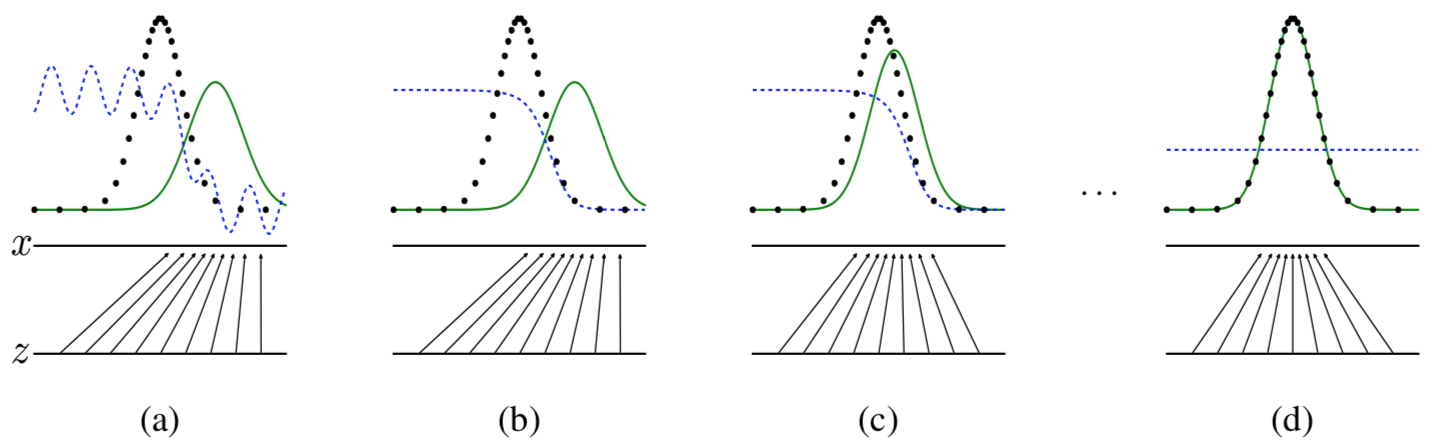
\includegraphics[width=\linewidth]{img/gan_training}
\caption{$p_{data}$ (black), $p_D$ (blue) and $p_G$ (green). Horizontal lines are (partial) domains of Z and X. Arrows show $G$'s mapping.}
\end{figure}
\pause
\begin{enumerate}[]
	\item a) distributions at start of iteration.
	\item b) updated $p_D$
	\item c) updated $p_G$
	\item d) The ideal post-training scenario: equilibrium, i.e. $p_{data} = p_{G} \land \forall X : D(X) = \frac{1}{2}$
\end{enumerate}
\end{frame}



\begin{frame}
\frametitle{`Face generation' using GANs}
\begin{figure}
	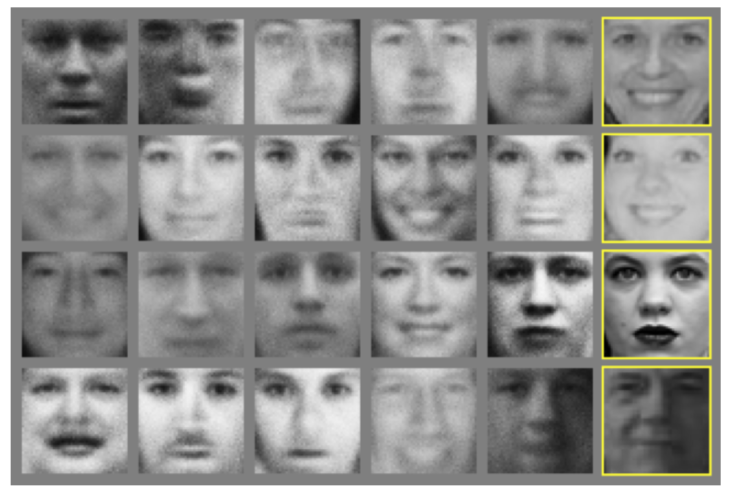
\includegraphics[width=\linewidth]{img/GAN_faces.png}
	\caption{Faces generated using GANs in original paper\cite{goodfellow2014generative}}
\end{figure}
\end{frame}



\begin{frame}
\frametitle{Problems with GANs}
\begin{itemize}
	\item Observation: at first, the difference between $p_G$ and $p_{data}$ will be huge. Effect:
	\begin{enumerate}[]
		\item $\nabla \mathcal{L}_G$ will be all over the place.
	\end{enumerate}
	\item Even more problematic for higher resolutions: initial difference between $p_G$ and $p_{data}$ will only grow.
	\item Idea: slowly increase resolution for both $G$ and $D$.
	\begin{itemize}
		\item $G$ will first learn macro aspects of $p_{data}$, e.g. a face always has two eyes.
		\item Add layers to $G$ and $D$ to slowly learn meso and micro aspects.
	\end{itemize}
\end{itemize}
\end{frame}



\begin{frame}
\frametitle{Progressive growing of GANs\cite{karras2017progressive}}
\begin{figure}
	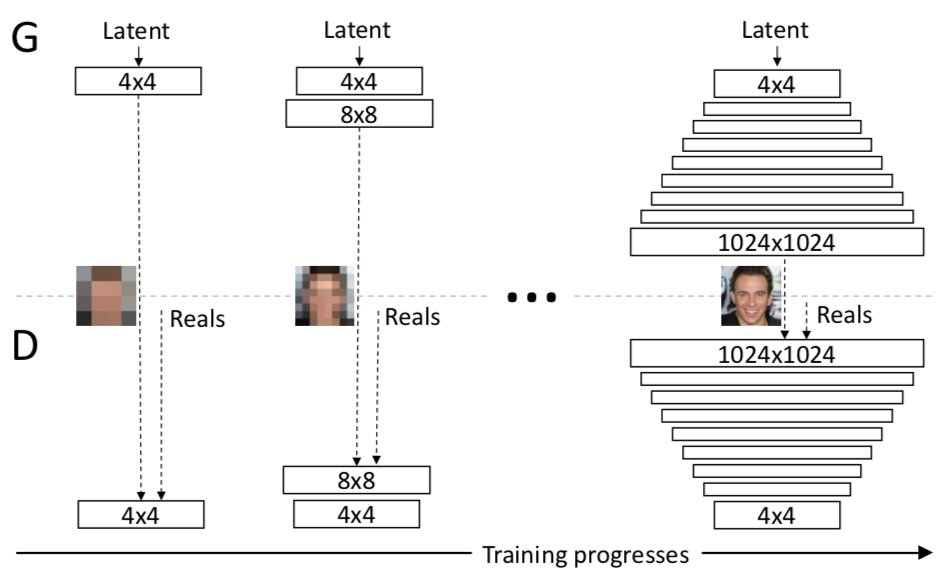
\includegraphics[width=0.8\linewidth]{img/prog_GAN.png}
	\caption{Visualisation of progressive growing of GANs.}
\end{figure}
\begin{itemize}
\item Latent vector size stays constant.
\item Training data is downsampled.
\end{itemize}
\end{frame}



\begin{frame}
\frametitle{Adding a new layer}
\begin{figure}
	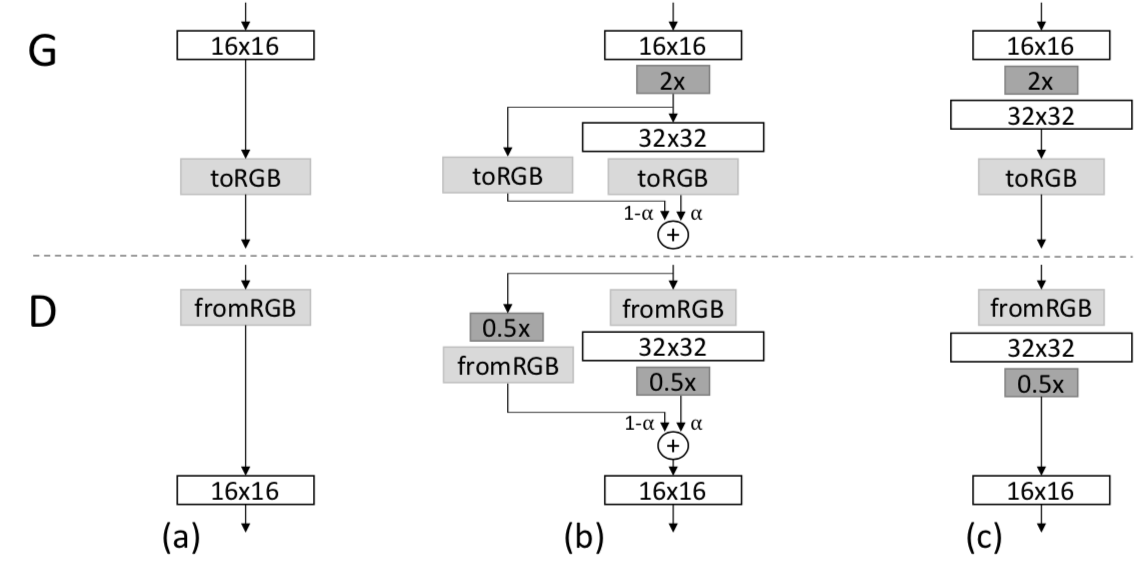
\includegraphics[width=0.8\linewidth]{img/prog_GAN_layer_add.png}
	\caption{Fading in a layer\cite{karras2017progressive}.}
\end{figure}
\begin{itemize}
	\item Upsampling: nearest-neighbour interpolation
	\item Downsampling: average pooling
	\item $\theta$ for new layer is initialised randomly.
	\item $\alpha$: linear transition parameter.
\end{itemize}
\end{frame}



\begin{frame}
\frametitle{Progressive growing of GANs\cite{karras2017progressive}: results}
\begin{figure}
	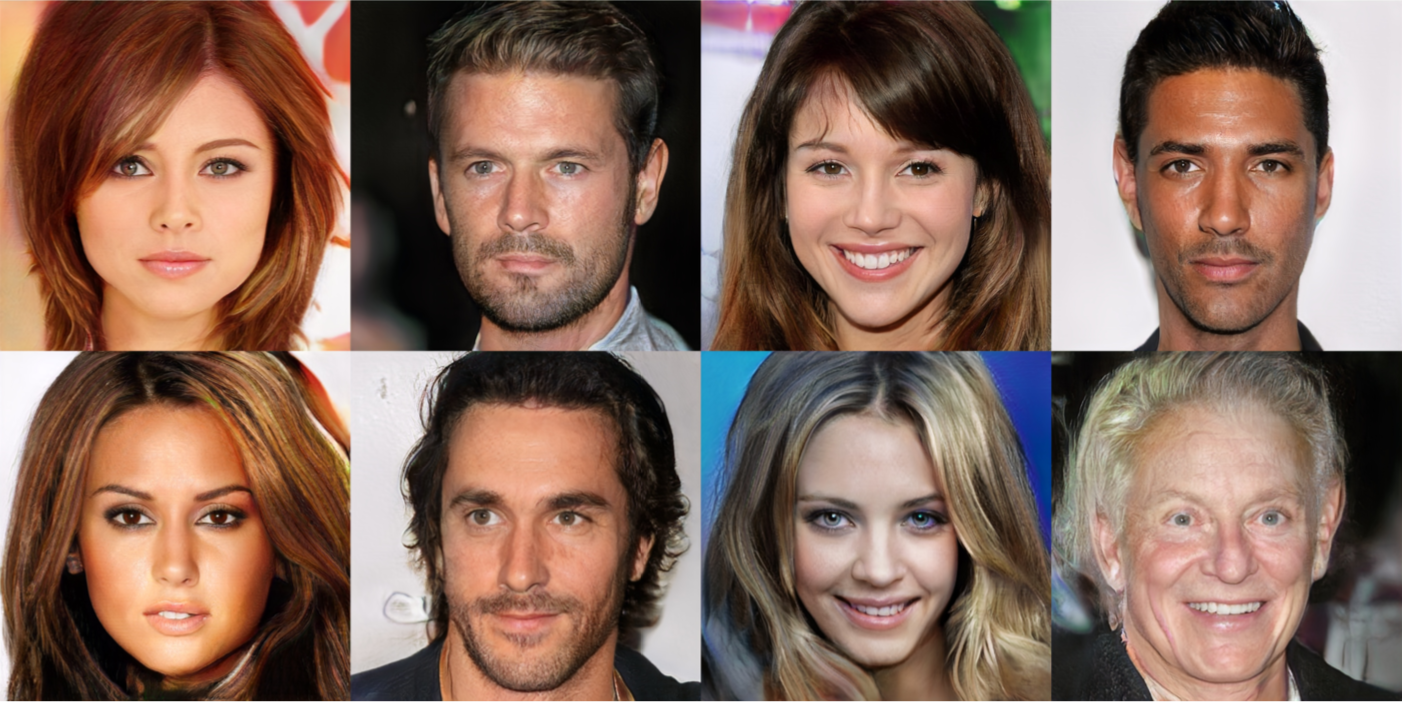
\includegraphics[width=\linewidth]{img/prog_GANs_celebs.png}
	\caption{`Celebrities' generated using a progressive GAN}
\end{figure}
\end{frame}



\begin{frame}
\frametitle{How random is the final $G$?}
\begin{figure}
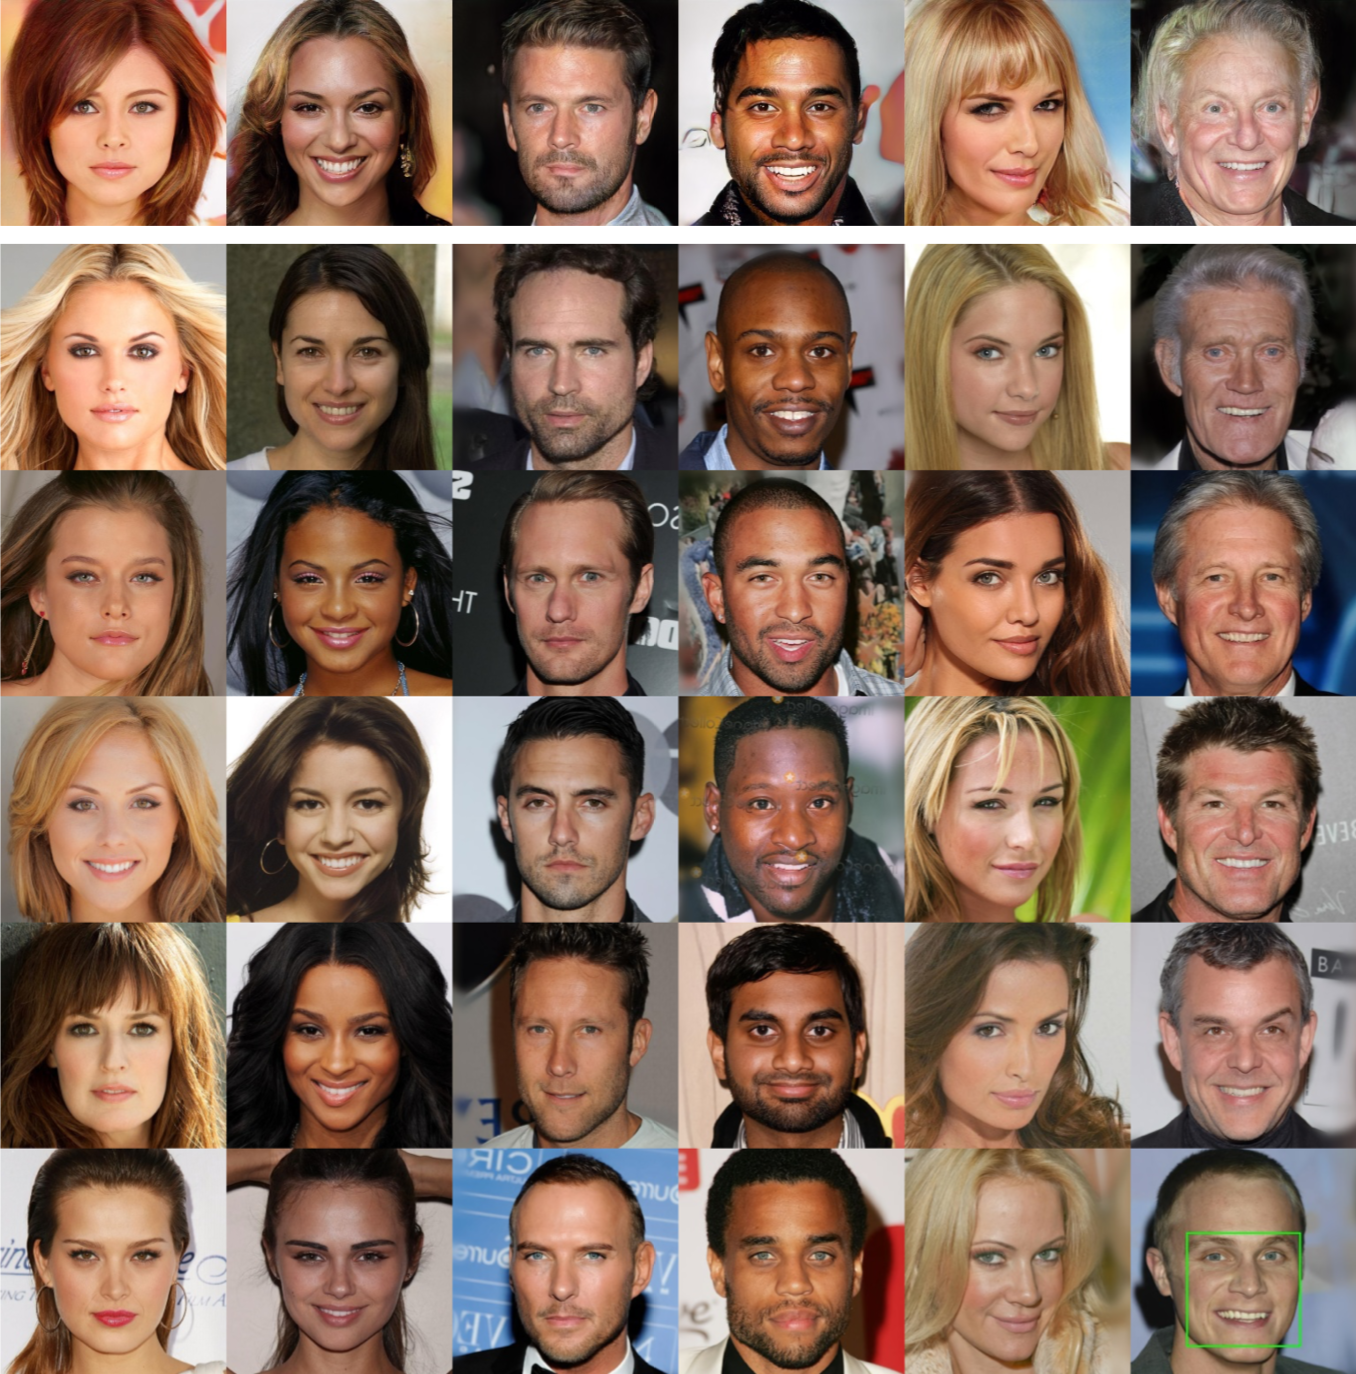
\includegraphics[width=0.7\linewidth]{img/prog_GAN_nn.png}
\caption{Nearest neighbours of the generated faces in the training set.}
\end{figure}
\end{frame}



\begin{frame}
\frametitle{Different ages}
\center{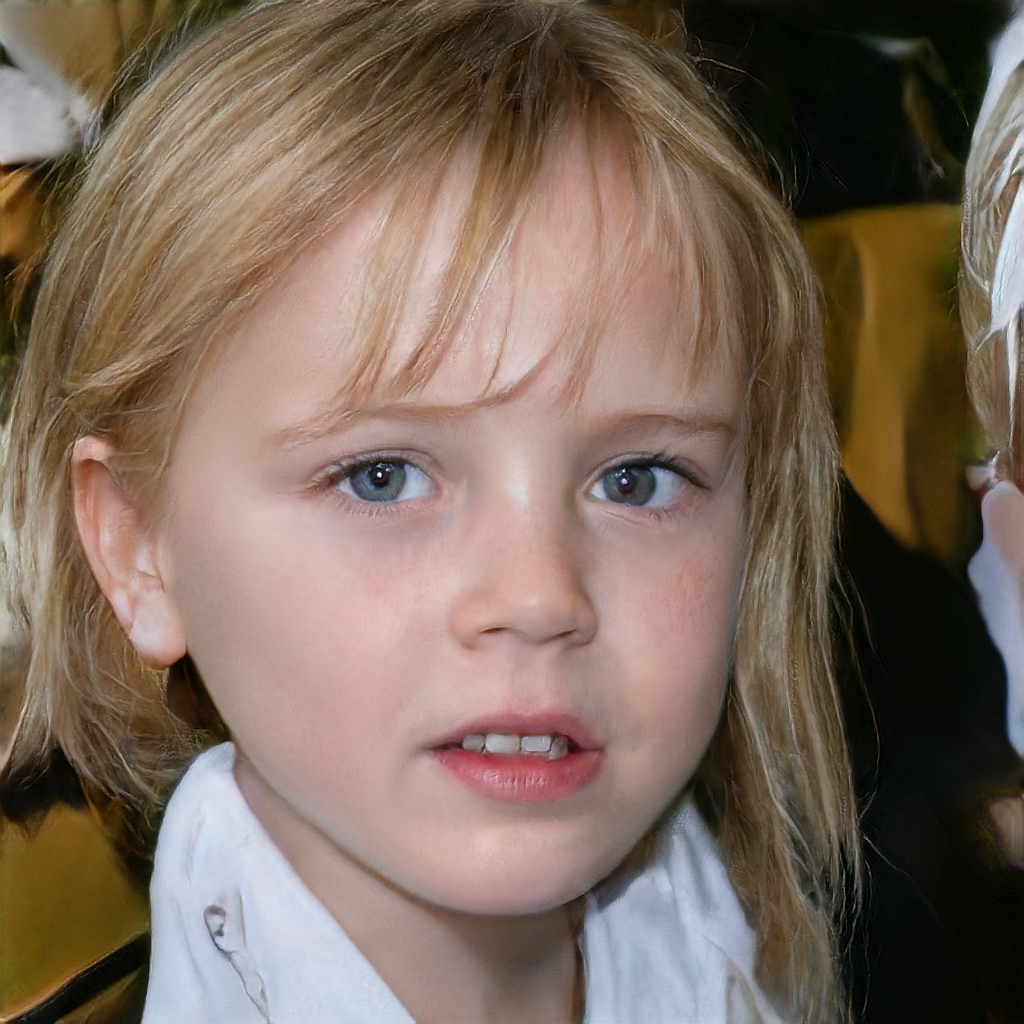
\includegraphics[width=0.65\linewidth]{img/f2}}
\end{frame}



\begin{frame}
\frametitle{Mistakes}	
\center{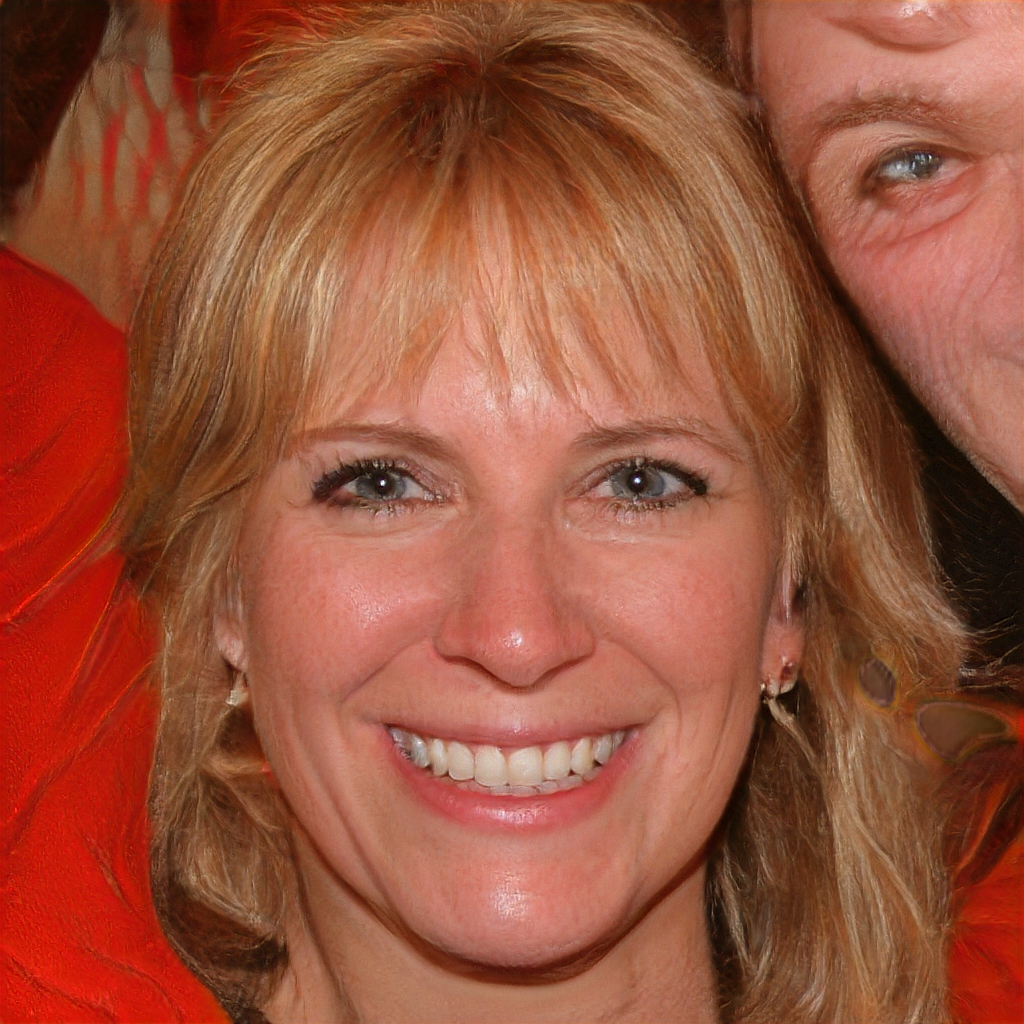
\includegraphics[width=0.65\linewidth]{img/f1}}
\end{frame}



\begin{frame}
\frametitle{Bonus: interpolation of latent input}
\movie[autostart]{\url{https://youtu.be/XOxxPcy5Gr4?t=107}}{img/latent_interpolation.mp4}
\end{frame}



\begin{frame}
\frametitle{Approaches}
\begin{enumerate}
	\item Autoregressive (AR) models:
		\begin{itemize}
			\item High quality
			\item Extremely slow
		\end{itemize}
	\item Variational Autoencoders (VAE)
		\begin{itemize}
			\item Blurry
			\item Fast
		\end{itemize}
	\item Progressively grown Generative Adversarial Network (GAN)
		\begin{itemize}
			\item High quality
			\item Fast (only 1 GAN, progressively grown)
			\item Increased GAN training stability
		\end{itemize}
\end{enumerate}
\end{frame}






\begin{frame}
\frametitle{Thank you. Bibliography}
\bibliographystyle{unsrt}
\bibliography{bibliography}
\end{frame}

\end{document}
